\documentclass[12pt,a4paper,fleqn]{report}

%Packages :
\usepackage[utf8]{inputenc}
\usepackage[fleqn]{amsmath}
\usepackage{amsfonts}
\usepackage{amssymb}
\usepackage[left=3.5cm,right=2.5cm,top=2.5cm,bottom=2.5cm]{geometry}
\usepackage{graphicx}
%For using biblatex and babel packages at the same time
\usepackage{csquotes}
\usepackage[style=ieee,useprefix,citestyle=numeric-comp,backend=bibtex]{biblatex}
\bibliography{reference.bib}

\usepackage{tabularx}
\usepackage[english]{babel}
\usepackage{listings}
\usepackage{xcolor} % for setting colors
%%%%%%%%%%%%%%%%%%%%%%%%%%%%%%%%%%%
\graphicspath{ {immagini/} }


% set the default code style
\lstset{
    frame=tb, % draw a frame at the top and bottom of the code block
    tabsize=4, % tab space width
    showstringspaces=false, % don't mark spaces in strings
    numbers=left, % display line numbers on the left
    basicstyle=\footnotesize\ttfamily,% basic font setting
    columns=fullflexible,
    commentstyle=\color{green}, % comment color
    keywordstyle=\color{blue}, % keyword color
    stringstyle=\color{red} % string color
}
%For the quotes paragraphs
\usepackage{etoolbox}
\AtBeginEnvironment{quote}{\singlespacing\small}
%dependency
\usepackage{setspace}

%For pseudocode 
\usepackage{algorithm}
\usepackage[noend]{algorithmic}

%For c++ code

\usepackage{listings}
\usepackage{color}



%%%%%%%%%%%%%%%%%%%%%%%%%%%%
\begin{document}
%TITLE PAGE
\begin{titlepage}
\begin{center}
\huge{\textbf{University of Calabria}}\\
\begin{figure}[bt]
\centering
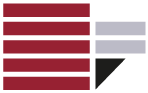
\includegraphics[scale=0.5]{Stemma}\\
\end{figure}
\line(1,0){400}\\[5mm]
\Large{\textbf{Department of Mathematics and Computer Science}}\\
\Large{\textbf{Bachelor Degree in Computer Science}}\\
\vspace{35mm}
\Huge{\textbf{Application of Distributed Discrete-Event Simulation Techniques in Parallel Execution of Cellular Automata}}
\end{center}
\vspace{35mm}
\begin{flushleft}
\large{\textsc{\textit{\textbf{ADVISOR}}}}
\hfill \large{\textit{\textsc{\textbf{EXAMINEE}}}}\\
\Large{\textit{Prof. William Spataro}}
\hfill \Large{\textit{Alessio Portaro}}\\
\Large{\textit{Prof. Donato D'Ambrosio}}
\hfill \Large{\textit{176231}}\\
\large{\textsc{\textit{\textbf{CO-ADVISOR}}}}\\
\Large{\textit{Eng. Andrea Giordano}}
\end{flushleft}
\vfill
\begin{center}
\line(1,0){430}\\[5mm]
{\large{\bf Academic Year 2018/2019}}\\
\end{center}
\end{titlepage}
%TITLE PAGE END
\newpage
\thispagestyle{empty}
\tableofcontents
\thispagestyle{empty}

\newpage
\setcounter{page}{1}
\chapter{Introduction}
%As suggested from the title, this thesis' main aim is to examine in depth some aspects of \textit{Cellular Automata} that may result in overhead reduction and performances improvements, when this kind of simulation is executed in a Parallel and Distributed Environment. Most specifically our focus will be on the notion of \textit{Idle Cell}, well known in CA's literature. Latter is strictly related with another concept, coming from Discrete-event Distributed and Parallel Simulation 
Nowadays, many entities operating in several fields, require some software or hardware utility to improve the results of their work. Among these utilities, some of the most interesting are the so-called \textit{Simulation Systems}, namely software frameworks, more or less complex, useful to handle and process great amount of data, concerning the same simulated model. Between the various applications, the followings are the most relevant ones :
\begin{enumerate}
\item
\textbf{Military simulators}, used to improve the effectiveness of the recruit's training. For instance there are many fly simulators to supplement the drills of pilots, or simulators to train soldier's strategy talent, which submit them battle scenarios and handle the evolution of the simulation starting from the soldier's answers.
\item
\textbf{Infrastructures simulators}, developed in order to monitor the behavior of some new technology or infrastructure's component. For example one could simulate the usage of a new communication protocol, or the impact, over a road network's traffic, of building a new transport highway.
\item
\textbf{Scientific simulations} are systems developed ad hoc to collect data in favour of some new theory or monitor the possible effects of a physical phenomenon, by the simulation of a model approximating its properties. I.e. in the next chapters of this treatise, it will be depicted a model which simulates the evolution of a landslide, by the simulation paradigm of a\\ \textbf{Cellular Automaton} : \textit{SciddicaT}.
\item
\textbf{Entertainment Industry }. In this field there are several applications and many others are to come, because of the great interest raised and all the heavy investments. One example that stands out among the others are the \textit{Augmented reality} platforms.
\end{enumerate}
 
The main categorization of the \textit{Simulation Systems} is in two opposite types, differing in the way the time flowing is modeled :
\begin{itemize}
\item
\textbf{Discrete-event simulation}, is a paradigm where the state of the simulation instantly evolves at certain points in time, while maintains its internal state between each couple of transition instants.
\item
\textbf{Continuous time simulation}, on the contrary is a paradigm where the simulation's state is supposed to change continuously during the time. The association between the state of the system and a point in the simulation time is kept via a mathematical function.
\end{itemize}
Both types of simulation are strongly related to the concept of time and the way the abstraction of the this last evolves during the system's evolution. In particular, in the case of the \textit{Discrete-event simulation}, which is the one we discuss in this thesis, there can be differentiated two main execution types, in accordance with the different ways the abstraction of the time evolves :
\begin{itemize}
\item
\textbf{Event-Driven execution} : When this paradigm of execution is adopted, the state of the system only changes when an event occurs, that's to say when an action would occur in the real system. Each event has to bear an unique time reference and usually affects the internal state of the system, generating new events itself. Whenever possible, this paradigm can be convenient because the simulator maybe doesn't perform useless operations, but could lead to a performance reduction in \textbf{as soon as possible} simulations.
\item
\textbf{Time-stepped execution} : This paradigm is characterized by the contemporary evolution of the system state and the time abstraction. The system makes the state evolve following a set of rules and increments the simulated time of a fixed quantity. As soon as the state change has been computed, the system starts the computation of a new step. A \textit{Time-stepped} execution could be convenient in a simulation to be executed in the shortest possible time.
\end{itemize}

\begin{figure}[ht!]
\centering
    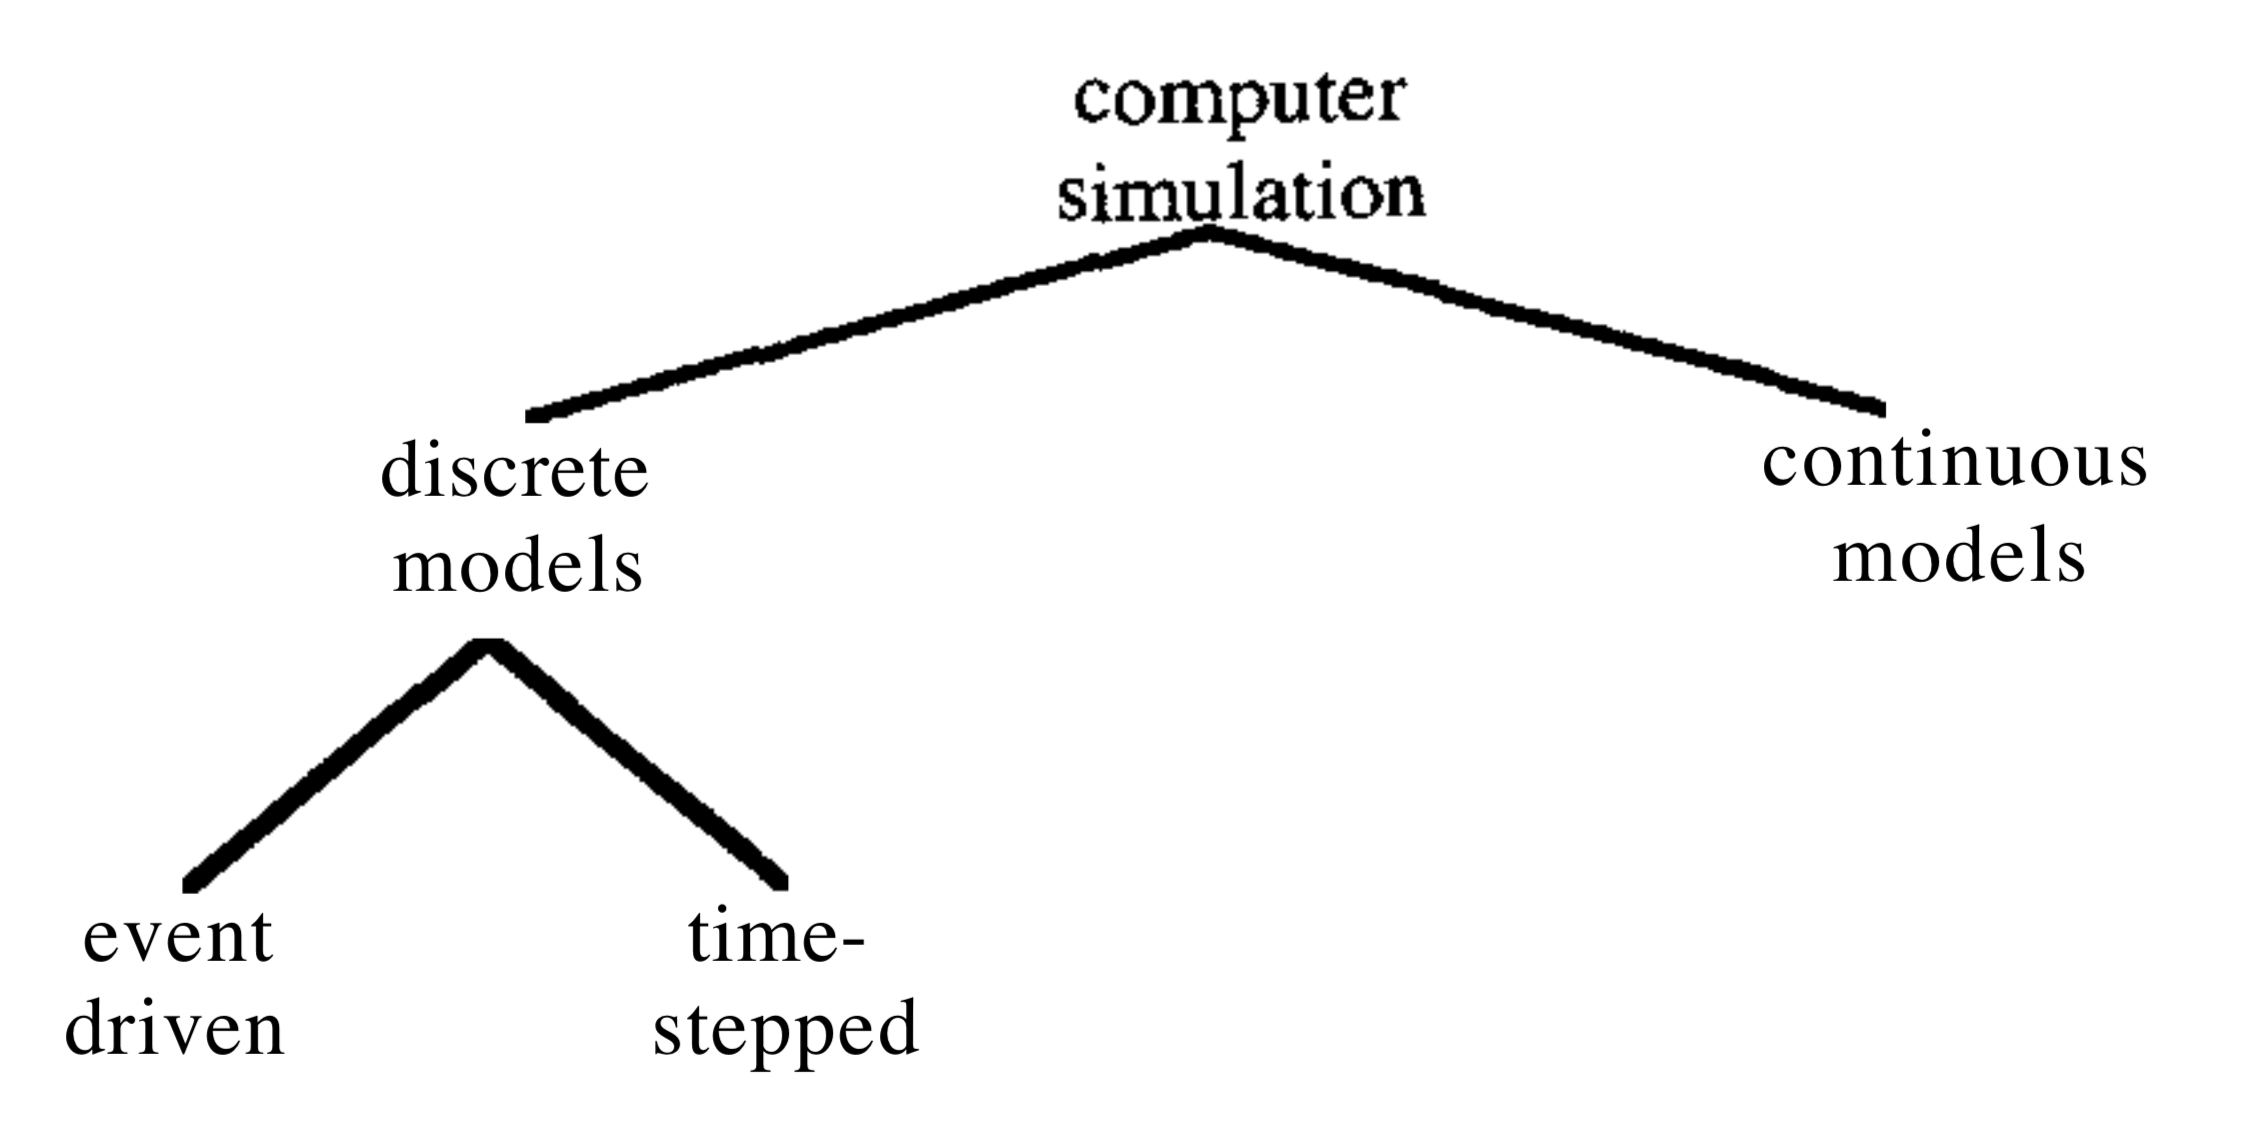
\includegraphics[width=0.75\textwidth]{simulation_paradigms}
    \caption{ Simulation systems classification \cite{0}  }
\end{figure}

One example of \textit{Time-stepped } execution is the \textbf{Cellular Automata} model. This simulation paradigm, often used to model natural processes,  provides for a data structure representing the physical space, composed of a huge amount of \textit{Cells} which evolve following the same fixed rules. Because in this kind of simulation, the main aim is to make the execution as fast as possible and because of how a \textit{Cellular Automaton} evolution works, the most intuitive way to increment the performance is to split the huge amount of elementary computations concerning all the \textit{Cells} into the space, between multiple CPUs, so that the execution is performed in parallel and in minor time. However the parallelization of the execution entails some overhead, coming from the resolution of the problems resulting from the distribution process, one of whom is the information exchange between the parallel CPUs, needed to make evolve the \textit{Cells} on the \textit{Borders} of their space portions. The just mentioned communication is often performed using the \textbf{MPI} technology, which is an \textit{API}, standard de facto for parallel applications which are designed to follow a message passing model. In the literature of the \textit{Parallel and distributed discrete-event} simulation systems, there are many general valid solutions that could be applied to the specific case of \textit{CA}. One of the most interesting concepts in this literature is the \textbf{LookAhead} applied to the \textbf{Synchronization Problem}. This problem occurs when two parallel processes, running portions of the same simulation, can invalidate their executions each other, affecting their respective simulated past, that's to say creating events with a timestamp minor then the actual value of simulated time. The \textit{LookAhead} is a concept whose understanding is necessary to solve the problem, because it is a value which ensures to each parallel process, a lower-bound, in terms of simulated time, to the timestamp of the next event that could affect its simulation. \\
As suggested from the title, this thesis' main aim is to examine in depth some aspects of \textit{Cellular Automata} that may result in overhead reduction and performances improvements, when this kind of simulation is executed in a Parallel and Distributed Environment. Most specifically our focus will be on the notion of \textbf{Idle Cell}, well known in CA's literature and the just mentioned \textit{LookAhead}. Using these two concepts, it has been tried to come out with an algorithm to reduce the parallelization overhead.
\newpage
\chapter{Cellular Automata}
%Chp 2.1
\section{\textit{CA}'s definition}
Introduced by mathematician John von Neumann in 1940s, a \textit{Cellular Automata(CA)} is a discrete computational paradigm, studied in computer science, mainly used to simulate complex phenomenon whom behavior derives from the basic interactions of spacial units named \textit{Cells}. A \textit{CA}, as said before, is composed of a  data structure which represents the space where the simulated phenomenon takes place. This data structure, often a matrix, is composed of many elementary units named A \textit{Cells}, therefore this structure is called cellular space. The evolution of the entire simulation is strictly related to the evolution of  all its elementary spacial units. A \textit{Cell}'s evolution, for its part, is related to the application of certain rules at every step of the simulation. Even if the rules of a \textit{CA} can be applied to an infinitely extended space, in a real simulation most of the time the number of \textit{Cells} is finite. Every \textit{Cell} interacts with a relatively narrow number of other \textit{Cells} whom state affect its evolution. The set of \textit{Cells} which affect the evolution of every spacial unit depends on the \textit{Neighborhood} relation. Latter is bound both to the simulated model and the existing types known in literature, from which a modeler can choose. \\

\begin{figure}[ht!]
\centering
    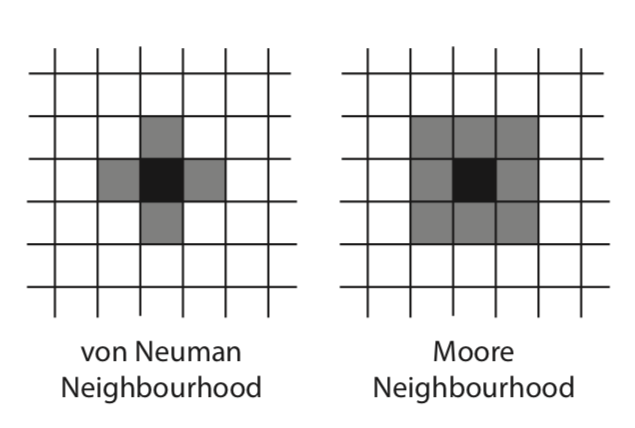
\includegraphics[width=0.5\textwidth]{neigh_types}
    \caption{  From the left to the right, Von Neumann and Moore Neighborhood  with radius equal to one \cite{1} }
\end{figure}

The \textit{Neighborhood} relation is a geometrical pattern, which relates a set of \textit{Cells}, fixed for every \textit{Cell} and every step of the simulation's evolution. The two most used types in literature, because of their simplicity and however effectiveness, are the following:
\begin{itemize}
\item
\textit{Von Neumann Neighborhood} : Fixed a number said radius, each \textit{Cell} in any direction whom distance from the one considered, for instance called C1, is minor or equal to the radius, is said to be in the \textit{neighborhood}, according to this definition.
\item
 \textit{Moore Neighborhood} : Fixed the just mentioned radius, for instance R, is said to be in the \textit{neighborhood} every \textit{Cell} whom all coordinates are distant from C1 at most R.
\end{itemize}


As said before, the evolution of every \textit{Cell} at a certain point of the simulation is uniquely given from the internal state and the state of the \textit{Neighborhood}. For each particular model there are a certain number of simple rules which have the aforementioned states as input and the next state of the \textit{Cell} as output. From this point of view, each \textit{Cell} evolves as a \textit{FSA (Finite State Automaton)}. Despite this simulation paradigm may seem trivial, it is still very relevant for getting to see the chaotic and complex evolution of the entire model at a macroscopic level.\\
Let's think about \textit{Conway's Game of Life}, a famous cellular automaton very studied in the 1970s. This is a two state and bi-dimensional automaton which elementary rules are the following :
\begin{itemize}
\item
A \textit{Cell} in the state \textbf{1} with a number of neighbors in the state \textbf{1} fewer than two goes to the state \textbf{0}
\item
A \textit{Cell} in the state \textbf{1} with a number of neighbors in the state \textbf{1} greater than three goes to the state \textbf{0} 
\item
A \textit{Cell} in the state \textbf{1} with a number of neighbors in the state \textbf{1} between two and three remains in the same state
\item
A \textit{Cell} in the state \textbf{0} with a number of neighbors in the state \textbf{1} equal to three goes to the state \textbf{1}
\end{itemize}
One of the most interesting aspects of this \textit{CA} is that from some randomized initial configuration of the \textit{Cells} in the simulated region, through its evolution this automaton shows the constant presence of some self-replicating structures, known as \textit{Gliders}, generating from some other structure type known as \textit{Gliders-Gun}. It can be proved that manipulating the initial configuration of the \textit{CA} to generate \textit{Gliders-Gun} and therefore \textit{Gliders}, in certain \textit{Cells} of the space, there will be certain interactions similar to computations. This aspect allows us to say that the aforementioned \textit{CA} can emulate a \textit{Turing machine}.\\
This example gives us an hint about \textit{CA} simulation paradigm's potentiality as well as it's capability of modeling complex systems behavior, starting from very elementary rules.
%Chp 2.2
\section{Parallel execution of \textit{CA}}
Since a \textit{CA}'s evolution consists of applying the same elementary rules (\textit{Transition Function}) to an huge number of \textit{Cells} in the simulation space, distributing the computation on many process in order to speed up the overall time of the simulation, may seem reasonable and easily workable. The most intuitive way to distribute \textit{CA}s is to split the cellular space in regular and contiguous portions and delegate the application of the \textit{Transition function} on each portion, to a process into the parallel environment. The subject's literature shows several ways of making such a split, depending on the topology of the \textit{CA}, its \textit{cells}'s shape and the dimensions of the cellular space. In fact the split can be made along one or more dimensions. The latter case can make the split more complex.

\begin{figure}[ht!]
\centering
    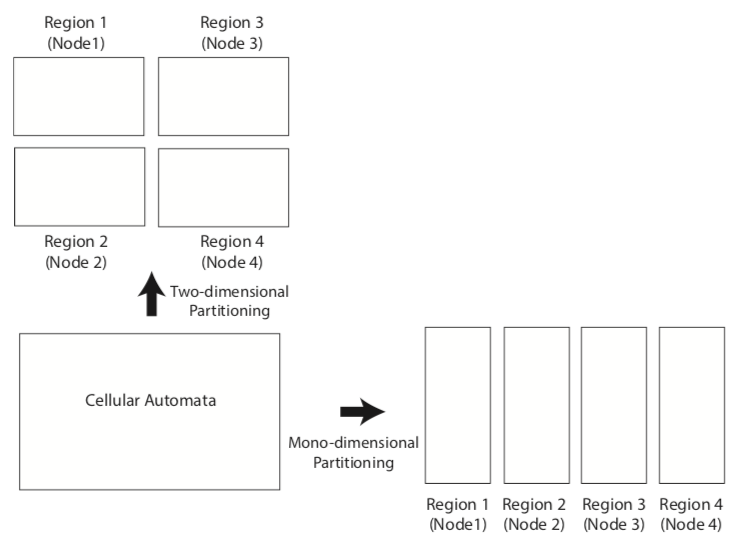
\includegraphics[width=0.5\textwidth]{split_types}
    \caption{  Some split examples : Mono-dimensional and Two-dimensional for a \textit{CA} with two dimensions and squared \textit{Cells} \cite{1}}
\end{figure}

Let's now think about the evolution of the \textit{CA} after being split and distributed to various processes, and let's focus on what happens for a \textit{Cell} close to the cut of the split that as been made. The informations about the \textit{Neighborhood} of such \textit{Cells} are located partly in the process which makes it evolve, but the remaining part is missing. In fact some of the \textit{Cells}'s  informations are located into that processes which have been delegate of apply them the \textit{Transition Function}. This trait is effective for every \textit{Cell} along the aforementioned cut. It is therefore reasonable to address the entire set of \textit{Cells} with this property and whom \textit{Neighborhood}s reside into the same process with a proper name : \textit{Border}. The process containing the \textit{Border} and the one containing the \textit{Neighborhood} of it's \textit{Cells} are said to be adjacent processes. 

\begin{figure}[ht!]
\centering
    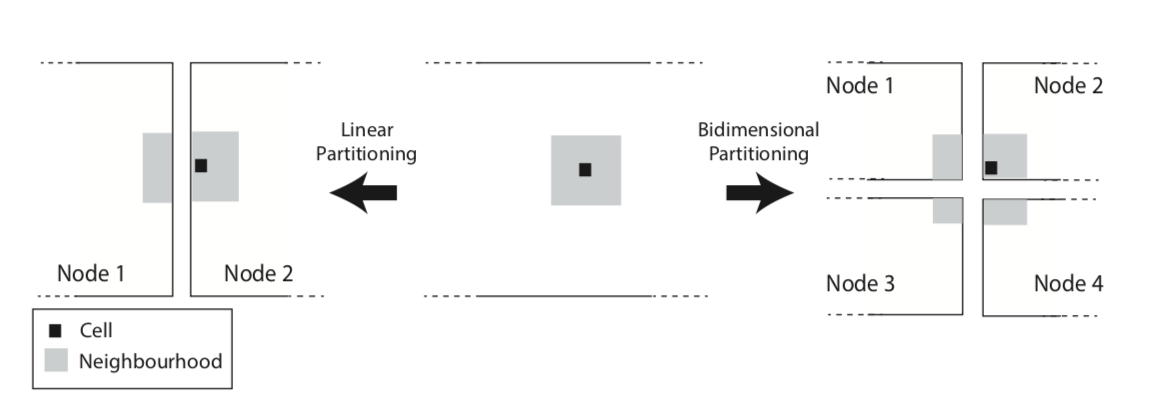
\includegraphics[width=0.75\textwidth]{missing_neigh}
    \caption{  Missing \textit{Neighborhood} of a \textit{Cell} along the cut \cite{1}}
\end{figure}

Because of the lack of information, before every discrete step of the simulation an interchange of information is required between every couple of adjacent processes, each sending his \textit{Border} and receiving another one from the respective coupled process. 

\begin{figure}[ht!]
\centering
    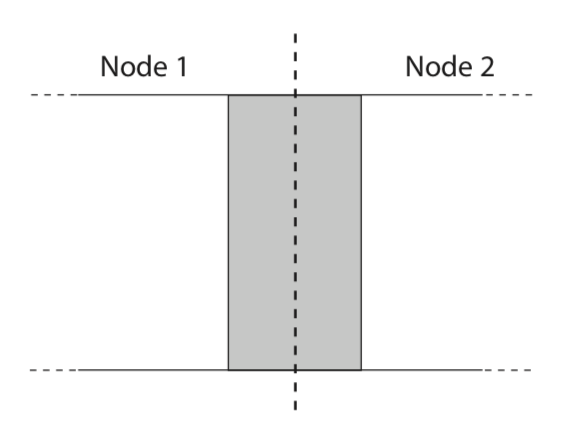
\includegraphics[width=0.5\textwidth]{border}
    \caption{  Example of a couple of processes and their related borders \cite{1}}
\end{figure}

This preparatory operation, before the application of the \textit{Transition Function}, introduces a performance's overhead strictly bonded to the parallel distribution of the computation. If such overhead could be avoid or just reduced, the performance gain resulting from the parallelization would be higher. The main aim of the study that is going to be shown in this thesis, is to find out some algorithm to exactly temper the mentioned overhead and obtain the related performance gain. 



%Chp 2.3
\section{Technologies and Frameworks }
As we have seen the interchange of \textit{Borders} between processes, is suitable for a communication paradigm that uses messages. To implement this communication, has been chosen to use the well known \textit{MPI(Message Passing Interface)} technology. It was designed as a language independent API (Application Programming Interface), in order to increase the portability of the applications using this technology, but however it has various implementations in many programming languages, among which the \textit{C++} version was used in the implementation of the conceived mechanism. \textit{MPI} is a standard for the communication of nodes in a cluster and is often used for high performance computing. The nodes in the cluster are often addressed as "processes" or "logical processes" and are grouped in so-called \textit{Communicators} within which they are arranged along various topologies. The processes in this topology mainly talk in point-to-point (\textit{p2p}) mode, and both blocking and non-blocking two-side communications are used. The main two couples of blocking and non-blocking methods are respectively \textbf{MPI\_Send - MPI\_Recv} and \textbf{MPI\_Isend - MPI\_Irecv}. When a non-blocking approach is chosen, at a stage of reception of the messages, a process has to be able to test or be notified when the operations are actually completed. One of the possible ways to perform such test of reception, is to use the method \textbf{MPI\_Iprobe}, which ,without blocking the execution flow, samples the message receiving. In order to perform a \textit{p2p} communication, each of the interlocutors has to know the ID of the other one within the \textit{communicator}. Moreover the data type of the informations to be transmitted have to be agreed. In addition to all the native types, corresponding to the native types of the majority of the programming languages, the standard MPI-1.2 provides for the definition of new data types (\textbf{MPI\_Datatype}). 
\\Thanks to this and other technologies, over time have been developed many frameworks for the parallel execution of \textit{CA}. Some examples of frameworks, developed at the \textit{"University of Calabria"}, are the following :
\begin{itemize}
\item
\textit{OpenCAL} : Modeling system for \textit{CA}
\item
\textit{libAuToti}: Library for \textit{CA} implementation using MPI
\item
\textit{CAMELot}: Parallel development environment for \textit{CA}
\item
\textit{VinoAC}: Framework for transparent execution of \textit{CA} in parallel and distributed environment, using \textit{MPI}
\end{itemize}
Among these frameworks, \textit{VinoAC} is the one that has been expanded with a module that, as said before, tries to temper the overhead caused by the interchange of \textit{Borders} and obtain a gain in performance terms.

\section{\textit{Cellular Automata}  applications}

Like it has been pointed out before, even in the \textit{CA} case there are many useful applications, some of whom are particularly fitting for this model, despite another simulation paradigm could also be used. The introduction of this report illustrates several examples of fields where the usage of a simulation system could be advantageous. However, again, not each of that examples are befitting for the  \textit{CA} paradigm, so here are the most appropriate ones:
\begin{itemize}
\item
\textit{Cryptography} 
\item
\textit{Artificial Life}
\item
\textit{Scientific Modeling}
\end{itemize}

____RIPRENDI DA QUI ____

\newpage
\chapter{\textit{D}istributed discrete-\textit{E}vent \textit{S}imulation }{\Large{\textit{DES}}}\\
%Chp 3.1
\section{Parallel Environments and Execution paradigms}
Even if the main aim of this research work was to think up to an algorithm, ensuring the consistency of the simulation's results and a good speed-up,  without hardware or software constraints, so that it can be as much generally strong as possible, sometimes certain assumption on the parallel environment's characteristics have turned necessary. It can be useful for this reason to get a quick overview of the primary traits which distinguish a parallel environment, in order to later understand the development choice that have been made. \\
First of all let us talk about the several possible hardware platforms. The main categorization differentiates the following machines, in the way all the informations are stored :
\begin{itemize}
\item
Shared memory Multiprocessors : Multiple processors share the same physical memory, hence every change to the data is visible to the other processors immediately
\item 
Distributed memory Computers : Multiple computers often heterogeneous have their own memory. If one of the computer modifies some data in its own local memory, and some other one needs exactly that data, some kind of message exchange is need. For this kind of architecture is very common the employment of general purpose connection networks rather than some customized one. This results in much more latency for the communication
\end{itemize}
More targeted architectures exist and have better performance than those aforementioned, however it doesn't make any sense to talk about an algorithm for such architectures here.
\newpage
\begin{figure}[ht!]
\centering
    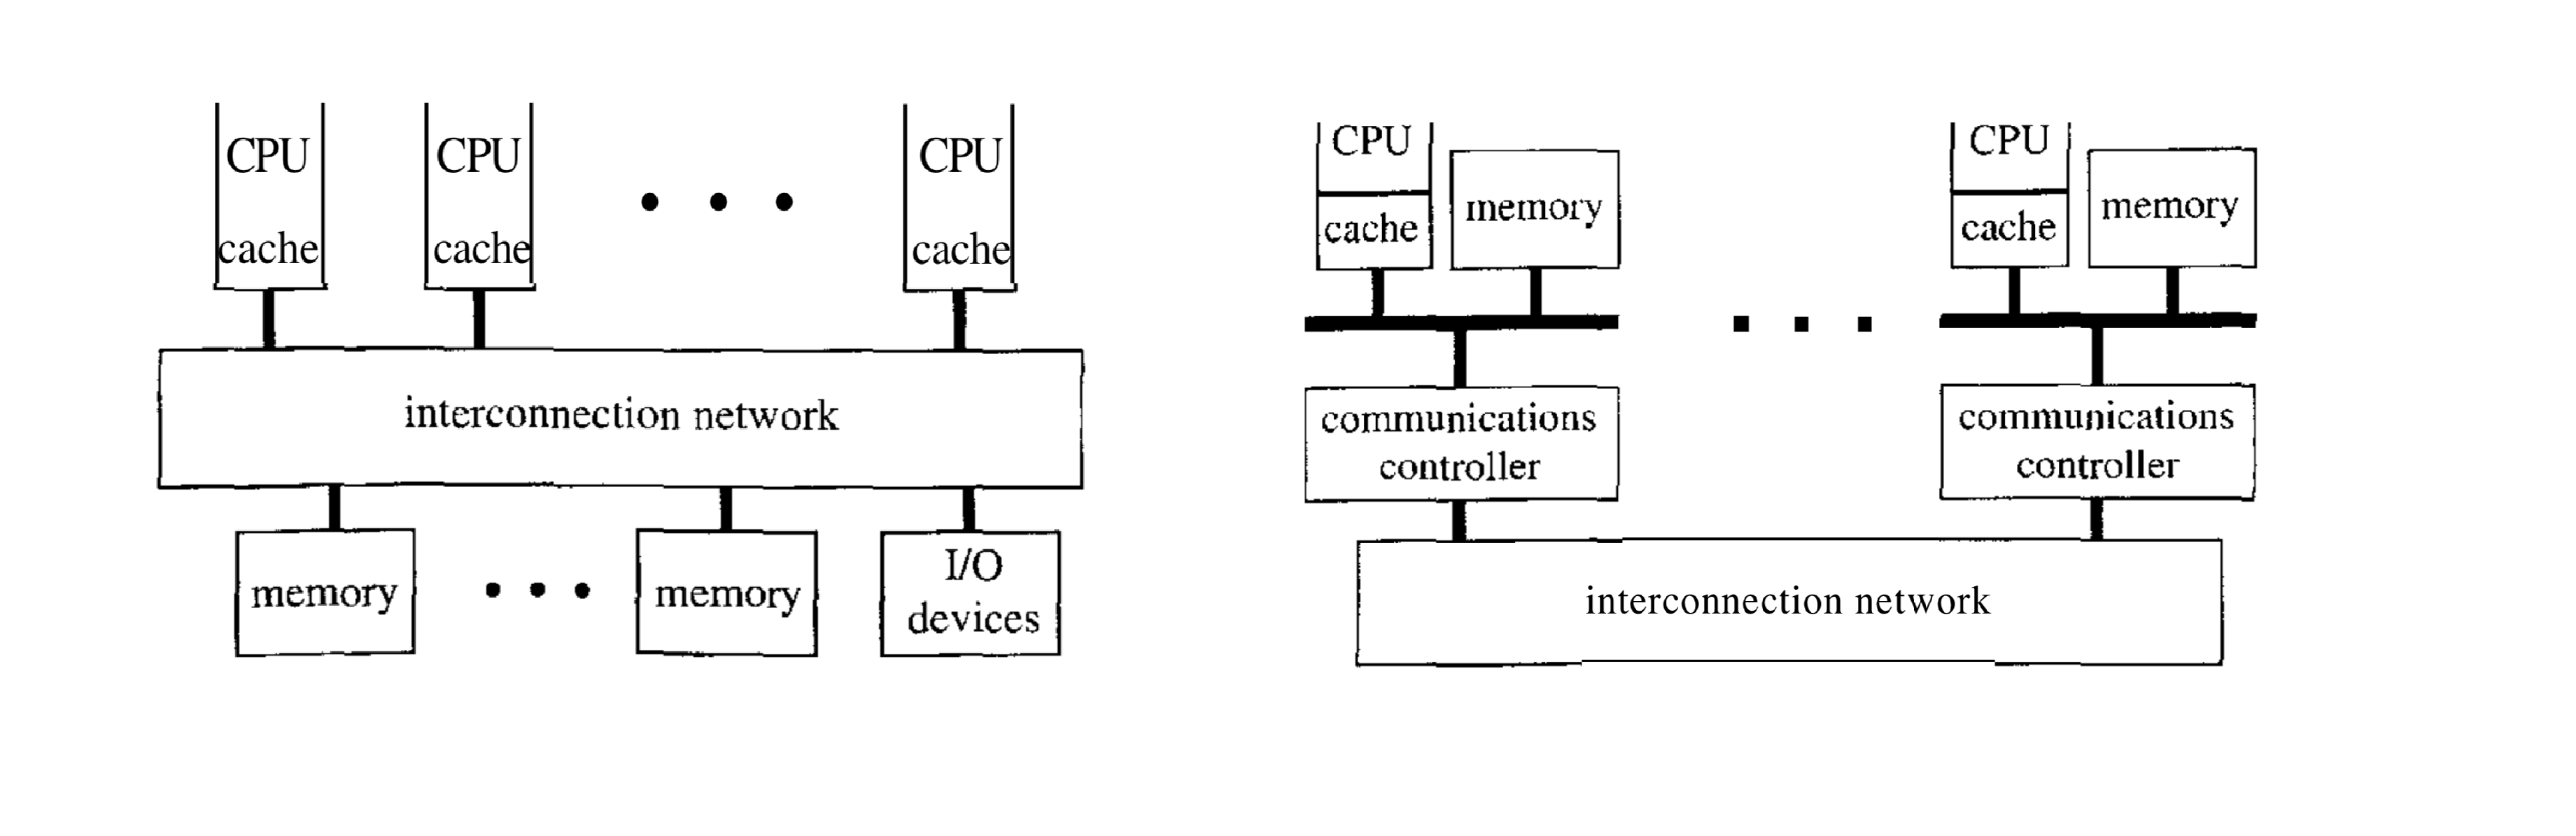
\includegraphics[width=0.95\textwidth]{parallel_architectures}
    \caption{  From the left to the right, shared memory multiprocessors architecture and distributed memory computers architecture \cite{0}}
\end{figure}
%FIGURA 
In second place, we can categorize the various paradigms for the parallel execution of a program, which can be summarized in these types :
\begin{itemize}
\item
\textit{SPMD(Single Program Multiple Data)} : The same executable is launched multiple times and different data in input (often one of these is some process ID)
\item
\textit{MPSD(Multiple Program Single Data)} : For every kind of task, a targeted program is created
\item
\textit{MPMD(Multiple Program Multiple Data)} : Less used paradigm, arrangement of the first two in this list
\end{itemize}
The parallel environment whom this text will refer from now on, belongs to the category of the Distributed memory architectures and uses the SPMD paradigm execution, even more because the latter is used in many \textit{C++} implementation of the \textit{MPI} technology, considered in the previous chapter. \\
	Besides the one made before, a further observation about the communication network concerns the reliability and the keeping of the sending order. In the conception of the algorithm, purpose of this work, it has been assumed a 100\% reliability of the connection network between the processes in the parallel environment, as well as it has been assumed that, traversing the network, the sending order of the messages doesn't change. This trait will result clearly important in the next chapter.
%Chp 3.2
\section{Discrete Event Simulation}
The \textit{Discrete-Event Simulation} paradigm's attempt, is to model the evolution of some real system with a chain of consecutive states, which stay unvaried for a definite amount of time preceding an instant when the system is thought to evolve immediately and enter in a new unchanging state. In this context the temporal dimension is very important to uniquely identify the state of the simulation, but it turns out to be necessary to give a definition of all the different "kinds" of time that can be encountered in the treatise. In the literature \cite{0} there are the following definition, which are really relevant for the considerations that are going to be \\
made :
\newpage

\begin{itemize}
\item
\textit{Physical Time} : Is the amount of time that would have elapsed, between two events or instants during to phenomenon being simulated, into the real world
\item
\textit{Simulated Time} : Is an abstraction of the \textit{Physical Time}, used inside the computer context to remark the state of the simulation's evolution
\item
\textit{Wallclock Time} : Is the amount of time taken from a machine to perform all of the necessary computations to make the simulation evolve to a certain \textit{Simulated Time}. Obviously the latter quantity depends on the hardware executing the aforementioned computations
\end{itemize}
Related to the disambiguation of the overlying terms, it may be useful to briefly examine how the \textit{Simulated Time} can be handled, in terms of how fast but also what is the reason of its increment. The main partition, concerning the haste of the simulation's execution, is into : 
\begin{itemize}
\item
\textit{Real time Simulation} : This kind of simulation needs the human interaction, maybe waiting for some input or simply a check. A military simulation, targeted for an airplane's pilot, may be an example of application where this approach is necessary, even if it slows down the execution time
\item
\textit{As fast as possible Simulation} : When the simulation doesn't need any kind of external input, but the main purpose is to speed-up the execution, in those cases this approach is the most appropriate 
\end{itemize}
Totally clear from the above partition, is the one concerning the reasons of every discrete state's change. In fact depending on the model being simulated, a simulation is said to be :
\begin{itemize}
\item
\textit{Event driven} if the events internal or external to the simulation, cause a change to the state and the \textit{Simulated Time}
\item
\textit{Time stepped}, more suitable for an execution \textit{As fast as possible}, if the simulation doesn't need any input to evolve and therefore when a state is completely set, the next one can be computed
\end{itemize}
A \textit{Time stepped} approach seems befitting for a \textit{CA} model, because its evolution consists of reading the state a the step \textit{t} of the \textit{Simulated Time} and then compute the state of the \textit{CA} at the time \textit{t+1}, without any other requirement.
%Chp 3.3
\section{The synchronization problem and lookahead}
As previously occurred in this treatise, when a sequential algorithm is transposed into a parallel environment, then some problem to be solved comes out. That's exactly the case for a \textit{Discrete Event Simulation}'s parallelization. \\
For instance in a Distributed environment containing heterogeneous machines, it is not that difficult to find out that at a given instant in the \textit{Wallclock Time} two different processes have reached different points into the \textit{Simulated Time}. Let's call this two processes \textbf{Lp1}(standing for \textit{Logical process}) and \textbf{Lp2}, and let's say Lp1 has reached a point into the \textit{Simulated Time} successive to the point reached from Lp2. If Lp1 and Lp2 can respective computations, the discrepancy between the \textit{Simulated Time} instants could be a problem, when Lp2 affects Lp1 in its past. Lp1 in fact would need to handle that event which potentially could have changed its state if it had arrived earlier in the \textit{Wallclock time}. In this case Lp1 is said to violate the \textit{Local Causality Constraint}, defined in literature as follows :
\begin{quotation}
\textit{Local Causality Constraint} : A discrete-event simulation, consisting of logical processes (LPs) that interact exclusively by exchanging time stamped messages obeys the local causality constraint if and only if each LP processes events in non-decreasing timestamp order \cite{0} 
\end{quotation}

To obviate to this issue one has to come up with some algorithm to prevent a situation like the one mentioned. The algorithms solving this problem can be categorized in two groups : 
\begin{itemize}
\item
\textit{Conservative approach} : An Lp can wind on only if it has the assurance to not receiving any message or event that could affect its past states
\item
\textit{Non conservative approach} :  An Lp planning to not receive anything affecting its past can wind on, but has to perform a roll-back operation if receives such a message or event
\end{itemize}
When a \textit{Conservative approach} is chosen an Lp at an instant \textit{t} can process an event with a timestamp \textit{t+l1} or make the simulation advance to the step \textit{t+l2}, only if it is sure that nothing with a timestamp less then \textit{t+l1} or \textit{t+l2} will be received. To make such assumption an Lp must have enough information about which other Lps in the simulation can affect its execution an particularly the value of the so-called \textit{Lookahead}. The latter is defined as follows :
\begin{quotation}
\textit{Lookahead} : If a logical process at simulation time \textit{\textbf{T}} can only schedule new events with time stamp of \textit{at least} \textit{\textbf{T+L}}, then \textit{\textbf{L}} is referred to as the lookahead for the logical process \cite{0}
\end{quotation}
To underline the relevance of this quantity, let us thing for instance to a situation when it equals zero. Under this condition an Lp cannot process any event or wind on to the next step because then it could receive a message violating the \textit{Local Causality Constraint}. In the next chapter the importance of this concept is going to result even more strong, when a parallelism with \textit{CA} paradigm will be drawn. 
\newpage
\chapter{Application of \textit{DES} techniques in Parallel execution of Cellular Automata}
\section{Synchronization problem for \textit{CA}}
As a first step of this research process, it has been tried to study the synchronization problem applied to the \textit{CA} paradigm in a parallel and distributed environment, in order to came out with some kind of \textit{Conservative} algorithm which could prevent the infringement of the \textit{Local Causality Constraint}, in a situation where every Lp handles a different automaton with its own time step, in terms of \textit{Simulated Time}. In that situation the different \textit{CA} would have been modeling different phenomena into the same complex system, and therefore would have been related to each other.\singlespacing Since also in this case an algorithm with the most general validity was wanted, the problem has been modeled around two main data structures. The first one is a dependency graph, dynamically configurable, which denotes for each Lp in the simulation, those which it can affect and those which can affect its own simulation. Let's call it \textbf{dependency\_graph}. Let this structure be composed by two lists, one containing the IDs of the Lps on which one depends, and the other containing the IDs of the Lps depending from it. Let's call the lists respectively \textbf{incoming\_arcs} and \textbf{outgoing\_arcs}. The second data structure is a vector containing the time step information. In particular, each Lp has two vectors, one containing the information about the Lps which depend from it, and a second one containing the information about the Lps on which it depends. It is important to say that just because of its connotation of general validity, any focus was given on the kind of information that a generic couple of processes has to exchange each other. The only constraint which is supposed to bound the evolution of every Lp, is that it has to receive from every Lp on which depends, its latest state informations as well as it has to send its own state information to let wind on the Lps which depend by it. Let's call the two vectors respectively \textbf{outgoing\_steps} and \textbf{incoming\_steps}.\\
After the element appearing in the algorithm being discussed, it's time to discuss its functioning as well. It will be used an example here, in order make the presentation of the algorithm easier. For instance immagine two processes Lp1 and Lp2 designated to make evolve in parallel environment, a couple of interdependent \text{CA}. Lp1 has a time step of 2 units meanwhile Lp2 has a time step of 9 units and depends on the first one. After a preparatory informations exchange at the \textit{Simulated Time} 0, every process is ready to evolve at the next step, therefore Lp1's \textit{Simulated Time} goes to 2 while instead Lp2 goes to 9. Because of its dependency from Lp1, Lp2 now can't evolve to the next step until Lp1 reaches the greatest instant until it moves into the future of Lp2. Lp1 instead can safely advance to time step 8 with 3 transitions. After performing every transition both Lp1 and Lp2 update not only their own time reference but also a reference for every of their related Lps. In our case Lp1 updates a reference to the time of Lp2 and Lp2 updates a reference for Lp1's time. It is exactly for this reason that when Lp1 hits the time step at the \textit{Simulated Time} 8, knowing the time step of Lp2 read from the vector \textbf{outgoing\_steps} can say it needs to send its state's informations to Lp2 which is dependent from him. Symmetrically, for the same reason Lp2 can say that he needs to receive some information from Lp1 to be able to evolve. Subsequently to this informations exchange both Lp1 and Lp2 are able to procede with their own operations.
\begin{algorithm}
\label{alg:one}
\begin{algorithmic}
	\STATE /* \textit{Vector containing the step reached from }
	\STATE\ *\ \ \ \textit{every dependent Lp}
	\STATE\ */
	\STATE Simulated\_time\_outgoing{[N]}
	\STATE /* \textit{Vector containing the step reached from}
	\STATE\ *\ \ \textit{every Lp on which this one depends}
	\STATE\ */
	\STATE Simulated\_time\_incoming{[N]}
	
	\WHILE{\NOT SIMULATION\_END}
		\STATE Can\_do\_step = \TRUE
   		
		 \FORALL{ Lp \textbf{in} incoming\_processes}
			\IF {Simulated\_time\_incoming + incoming\_steps \textless MY\_CURRENT\_TIME}
				\STATE Can\_do\_step = \FALSE
			\ENDIF
		\ENDFOR
		
		\IF{Can\_do\_step}
			\STATE CA\_Transition()
			\STATE MY\_CURRENT\_TIME += step
			
			\FORALL{Lp \textbf{in} outgoing\_processes}
				\STATE MPI\_Isend(MY\_CURRENT\_TIME)
			\ENDFOR
		\ENDIF
		
		\FORALL{Lp \textbf{in} incoming\_processes}
			\STATE incoming\_message = MPI\_IProbe(Lp)
			\IF{incoming\_message}
				\STATE MPI\_Recv(Lp)
				\STATE Simulated\_time\_incoming += incoming\_steps
			\ENDIF
		\ENDFOR
		 
 	 \ENDWHILE
 	 
\end{algorithmic}
\caption{run\_simulation() \textit{Pseudo-code of the algorithm's main loop}}
\end{algorithm}

Like one can see from Algorithm \ref{alg:one}, in a real situation with a more complex dependency graph, thanks to the \textit{MPI}'s non-blocking functions \textbf{MPI\_Isend} and \textbf{MPI\_IProbe} any deadlock situation can be prevent. Furthermore, again thanks to \textit{MPI}, the algorithm doesn't need to implement any acknowledgment mechanism to make sure that every dependent Lp knows about the advancement of the simulation in another process because, as said before, the \textit{MPI} communication network can thought with a perfect reliability. \\
Even if this algorithm can be useful in certain situations, the effort to think up such a mechanism was minimal as well as it's minimal its scientific significance. In fact it doesn't profit by any of the aforementioned \textit{DES} techniques nor brings to any performance gain in the execution of such kind of simulation. The reason is that every \textit{CA} simulation can be categorized as a time-stepped simulation and moreover in usually it's evolution depends on its own internal state. A general mechanism as the one just described is meaningless if any assumption, about how the execution of a \textit{Cellular Automaton} can be affected, can be done. 
\section{\textit{Lookahead}'s study for border swap avoidance}

Things are different if we talk about the execution of a single \textit{Cellular Automaton} distributed through a parallel and distributed architecture. In this case in fact, every Lp which is assigned to make evolve a portion of the cellular space is inherently bound to the other Lps in the simulation. In this context, as seen in the section dedicated to the Parallel execution of \textit{CA}, every couple of adjacent Lps, has to permanently communicate, asking and being asked about their respective \textit{Borders}. Because of this, in the second phase of the study work, the main focus has been on finding a way to moderate the overhead due to that communication.\\ 
In particular an Lp containing a \textit{Border} that has not changed, in any of its cells, after applying the \textit{Transition Function}, in principle doesn't need to transmit that \textit{Border} again. Unfortunately there is an issue here regarding the possibility of run into a \textit{deadlock} situation. So, if for example an Lp skips a transmission, its adjacent interlocutor, which expects this information after every step of the evolution, will freeze its execution. Thus, a mechanism to let every the Lps know when to receive or send a \textit{Border} is needed. In other words each Lp needs a \textit{Lookahead} information about every of its adjacent interlocutors. However, to find a value for such information one needs to find some middle ground between a general valid concept and something dependent on the model. The middle ground was found into the \textit{CA}'s concept of \textit{Idle Cell}. A cell whom state doesn't change after applying the \textit{Transition Function} is said to be and \textit{Idle Cell}. This concept is particularly relevant if one thinks of the possible assumptions that can be done about the evolution of a \textit{Cell} with another \textit{Idle} one in its \textit{Neighborhood}. For instance it's not unreasonable to think that under certain conditions such \textit{Cell} could take two steps to change its state. Applying the same reasoning recursively to \textit{Cells} more and more distant from an active one, likewise the number of steps to change their state could grow up. In this way an Lp can find a value of \textit{lookahead} for its borders if considering the \textit{Idle Cells} in its own Cellular space and in its adjacent Lp's ones. It seems clear, from the previous arguments, that a \textit{lookahead} calculated with this assumptions, has to be directly proportional to the distance from the nearest active \textit{Cell} of each border.
\section{The starting point for the implementation}
Since, unlike in the first algorithm's event, in this case there are many frameworks already implemented which are delegated to run a \textit{CA} in a parallel and distributed environment, it was decided to use one of these as a starting point. Between several of these, it was decided to use the \textit"University of Calabria" 's framework named \textit{VinoAC}. In particular, this framework has been extended with a module whom functioning will be shortly explained. As said in the past chapters, \textit{VinoAC} is a framework for the transparent execution of a \textit{CA}. The modeler has only to specify its model's elementary rules and then to start the simulation, without caring about the internal mechanism which permit the execution. This framework was developed in \textit{C++}, thus it has an Object-oriented structure. Its architecture was designed to permit the usage of different parallel communication paradigms, but the only implementation to date uses the aforementioned \textit{MPI} paradigm. The three primary classes in the framework architecture\\
are the following :
\begin{itemize}
\item
\textit{\textbf{Model2D}} : This is an object containing all of the model's information. The framework provides a basic interface to be extended for every specific CA. After one overrides the class's method which represents the transition function the simulator can make the CA evolve.
\begin{lstlisting}[language=C++,
                   directivestyle={\color{black}},
                   emph={int,char,double,float,unsigned},
                   emphstyle={\color{blue}},
                   caption={Model2D.h, Interface to be implemented by the Modeler},
                   captionpos=b
                  ]
#ifndef MODEL2D_H
#define MODEL2D_H

#include <Space2D.h>

template <class T>
class Model2D
{
  protected:
    Space2D<T> *space;
  public:
    void setSpace(Space2D<T> *space);
    virtual void init() = 0;
    // Transition function of the (x,y) cell
    virtual void transitionFunction(int x, int y) = 0;
    virtual void finalize() = 0;
    virtual ~Model2D();
};
#endif
\end{lstlisting}
\item
\textit{\textbf{Space2D}} : This is an object whose job is to handle the cellular space. The modeler doesn't need to know if the cellular space is distributed in multiple processes or is computed in sequential. As we said before, the basic interface is designed to be implemented using different communication paradigms, but the one used from the conceived algorithm uses the \textit{MPI} paradigm. This object contains two matrix representing the cellular space. From the matrix \textbf{regionCurr} the simulator reads the current state of the \textit{CA} and applying the \textit{Transition Function} it writes the new state into the matrix \textbf{regionNext} and then calling the method \textbf{swap()}, the latter matrix is copied into the first one.
\newpage
\begin{lstlisting}[language=C++,
                   directivestyle={\color{black}},
                   emph={int,char,double,float,unsigned},
                   emphstyle={\color{blue}},
                   caption={Space2DMpi.h, Space handler using the MPI paradigm},
                   captionpos=b
                  ]
//Class for a two-dimensional CA space when the MPI technology is adopted
#ifndef SPACE2DMPI_H
#define SPACE2DMPI_H

#include <Space2D.h>
#include <Element.h>

template <class T>
class Space2DMpi : public Space2D<T>
{
protected:
  enum Direction  { N, NE, E, SE, S, SW, W, NW};

  int currentStep = 0;
  // Read matrix
  T *regionCurr; 
  // Write matrix
  T *regionNext; 
  
  void updateBorders();
public:

  void swap();
};

#endif
\end{lstlisting}

\item
\textit{\textbf{Engine2D}} : This is an object whose job is to pull together the two previous objects. It reads the informations from the model and then it changes the state of the \textit{CA}. After initializing the simulation, the method \textbf{start()} is called. This method contains the main loop of the simulation. 
\begin{lstlisting}[language=C++,
                   directivestyle={\color{black}},
                   emph={int,char,double,float,unsigned},
                   emphstyle={\color{blue}},
                   caption={Engine2D.h, The engine running the simulation and the main loop method},
                   captionpos=b
                  ]
#ifndef ENGINE_H
#define ENGINE_H

#include <Model2D.h>
#include <Space2D.h>


//Base class for the engine running a 2D cellular automata

template <class T>
class Engine2D{
    protected:
    // The CA space
    Space2D<T>* space;
    // The application model
    Model2D<T>* model;
    // The number of steps
    int nsteps;
    
public:

    void setSpace(Space2D<T> *space);
    void setModel(Model2D<T> *model);
    //Sets the number of steps
    void setNsteps(int nsteps);    
    void start(){
    	// Initialize the cellular space
    	model->init(); 
    
    	for (int step = 0; step < nsteps; ++step){
			space->setCurrentStep(step);
			// Initialize the step
			space->startStep(step); 
			for (int x = minX; x <= maxX; ++x)
				for (int y = minY; y <= maxY; ++y)
					// Apply the transition function to every cell in the space
					model->transitionFunction(x,y);
			// Write regionNext into regionCurr matrix
			space->swap();
		}
    }
};

#endif
\end{lstlisting}
\end{itemize}
This framework has been chosen as a starting point of the implementation phase of this work, due to its suitable architecture presenting a clear division between the \textit{CA}'s model and its cellular space. But, even if \textit{VinoAC} was a good starting point, some criticality were found into the \textbf{Space2D} class and in the way it handles the \textit{Borders} exchange.
\section{\textit{VinoAC}'s \textit{LookAhead} module}
Since \textit{VinoAC} implements the classic execution of \textit{CA}, the class \textbf{Space2D}, after each step of the simulation, takes care of the \textit{Borders} exchange between every couple of adjacent Lps. That's exactly why the first thing clearly to modify was this class and more specifically its method \textbf{startStep(int step)} which contains all the preliminary operations to each step of the simulation's evolution, including the \textit{Borders} communication. Secondly a way to know if a \textit{Cell} is \textit{Idle} seems necessary, therefore the base class \textit{Model2D} has been extended with the addition of a the method \textbf{bool isStanding(int x, int y)} by which it is possible to ask for such information to the specific \textit{CA} model. With these elements being given, the only remaining thing to do is to explain the main algorithm's functioning. \\
The algorithm consists of two parts, one which dynamically updates the lookahead value for each adjacent Lp of the one considered, during the application of the \textit{Transition Function}, and the other which handles the conditional exchange of the \textit{Borders} or some other related information. The second part is the one that's going to be explained first. \\
Consider as usual, two adjacent processes Lp1 and Lp2. Let's consider only the Lp1's point of view as a simplification in order to better understand the functioning of the mechanism. With this assumption we mean to say that Lp1 is the sender of the \textit{Border} whereas Lp2 is intended to only play as the receiver. Suppose also that in an initial phase both Lp1 and Lp2 know about the \textit{LookAhead} value related to the communication that they usually do at every step. From now on we'll refer to this value with the symbol \textit{LAh}. Considering what the \textit{LAh} value means, that's to say a promise that the \textit{Border}, known from both the Lps in an initial phase, won't change for the next \textit{LAh} steps, then an Lp can make evolve its portion of cellular space for that number of steps, saving itself the overhead caused by the usual communication operation. Obviously every both Lp1 and Lp2 are meant to decrement their local reference of the \textit{LAh} value after each step of the evolution, in order to contemporary reach a situation where the reference equals 0, meaning that the \textit{Border} well know until that moment could have changed and therefore the Lps need to perform some kind of communication to figure out what to do next. 
After reaching this point, Lp1 computes a new value of \textit{LAh}, which as known is a non-negative integer. Accordingly to the resulting value, a choice takes place : 
\begin{enumerate}
\item
If the \textit{LAh}'s value is strictly greater than zero, that means the \textit{Border} won't in effect change. It's important in fact to underline that the \textit{LookAhead} value in a context of general validity, is intended to represent only a lower bound for the real number of steps that a \textit{Border} needs to change. The modeler in effect could be unable to make such strong assumptions on the simulated phenomena to come out with an exact value of \textit{LAh}. Since it has this information, Lp1 notifies Lp2 that the \textit{Border} won't change sending a message with tag \textbf{LookAhead\_Update}, containing the new value. Lp2 after decrementing to zero its reference to \textit{LAh}, puts itself in listening of some message. Reading the tag of the message sent from Lp1 updates its reference of \textit{LookAhead} and resumes its execution.

\item
If otherwise the \textit{LAh}'s value equals zero, that means the \textit{Border} will change after the \textit{Transition Function} is applied. Therefore Lp1 sends a message with tag \textbf{LookAhead\_Update\_Following\_Border}, meaning that it will send the new \textit{Border} into the next step. Then, just after the \textit{Transition Function} is applied and the \textit{Border} has changed, Lp1 sends a message with tag \textbf{Border\_Update}, containing the new boundary informations. Lp2 which was waiting for a message, receives the one with tag \textbf{LookAhead\_Update\_Following\_Border}, applies the \textit{Transition Function} and then receives the new \textit{Border}.
\end{enumerate}
Thanks to this first part of the algorithm, an Lp which can compute the value of \textit{LookAhead} for each of its \textit{Borders} can improve its performance in the execution of the \textit{CA} moderating the overhead coming from the parallelization. It is clear that in a real situation each Lp has to communicate with several adjacent processes and it also has to play both the roles of \textit{Borders} sender and receiver. In order to avoid any \textit{deadlock} situation, even in this case the \textit{MPI}'s non-blocking functions fit our case. In fact, performing all of the send operations in non-blocking mode and then, playing the role of receiver, performing all of the receive operations, every Lp can avoid any kind of \textit{deadlock}.
\newpage
\begin{lstlisting}[language=C++,
                   directivestyle={\color{black}},
                   emph={int,char,double,float,unsigned},
                   emphstyle={\color{blue}},
                   caption={Space2DMpiLAh.h::\textbf{startStep(int step)}, implementation of the first part of the algorithm},
                   captionpos=b
                  ]
#ifndef SPACE2DMPILAH_H_
#define SPACE2DMPILAH_H_

template <class T>
class Space2DMpiLAh: public Space2DMpi<T> {
public:
void Space2DMpiLAh<T>::startStep(int step){
	//Two FOR cycles to avoid deadlock. The first one contains only non-blocking send
	for(int i=0;i<Neighbors_Number;i++){
		if(last_LAh_sent == 0){
			//To advance this Lp's neighbor needs some info about this Lp's border
			int new_lookahead = computeBorderLookAhead(i);
			if(new_lookahead>0){
				/* When the new_lookahead value is still greater then zero,
				 * it means the border sent in the past still won't change for
				 * at least LAh number of steps
				 */
				MPI_Isend(LOOKAHEAD_UPDATE);
			}
			else{
				MPI_Isend(LOOKAHEAD_UPDATE_FOLLOWING_BORDER);
			}
		}else last_LAh_sent--;
	}
	// Receiver loop
	for(int i=0;i<Neighbors_Number;i++){
		if(last_LAh_received == 0){
			//To advance this Lp needs infos about neighbor's border -> SEND
			
			while(true){
				MPI_Iprobe(LOOKAHEAD_UPDATE);
				MPI_Iprobe(LOOKAHEAD_UPDATE_FOLLOWING_BORDER);
				if(RECEIVED_LOOKAHEAD){
					MPI_recv(LOOKAHEAD_UPDATE);
					break;
				}
				if(RECEIVED_LOOKAHEAD_N_BORDER){
					MPI_recv(LOOKAHEAD_UPDATE_FOLLOWING_BORDER);
					
					MPI_recv(border);
					break;
				}
			}
		}else last_LAh_received--;
		}
	}
}

};

#include "Space2DMpiLAh.ipp"
#endif /* SPACE2DMPILAH_H_ */

\end{lstlisting}
\newpage
The assumption of the discussed mechanism however, remains the computation of the \textit{LAh} value. As said before the \textit{LookAhead} is a quantity supposed to be, in the \textit{CA}'s case, proportional to the distance between those \textit{Cells} which are not \textit{Idle}, and the \textit{Border} of the cellular space's portion assigned to an Lp. \\
After underlining that even the proportionality above is an implementation choice, that could be invalidated in certain cases, we can say that for simplicity and for the purpose of letting the algorithm apply in general, it has been chosen to make the \textit{LookAhead} exactly coincide with that distance value. This chose allows to maintain the lower-bound connotation of the \textit{LAh}, compared to its computation as a quantity proportional to the distance, meaning it would have been a greater value. Because of the data structure used to represent the cellular space, that's to say a two-dimensional matrix, the computation of a distance occurs with constant time complexity (\textbf{\textit{O(1)}}), thanks to the indexing of every element in such data structure. Since the \textit{LookAhead} is a lower-bound to the number of steps needed from a \textit{Cell} on the \textit{Border} to become active and therefore change, requiring another \textit{Borders} exchange, then its value has to be computed as the distance between the nearest not \textit{Idle Cell} and each border. The crucial point is then to detect the nearest active \textit{Cell}. In order to do find this \textit{Cell}, each Lp has to iterate all over its portion of cellular space. Such iteration is also performed during the application of the \textit{Transition Function}, therefore one can take advantage of that and during this iteration check whether a \textit{Cell} is \textit{Idle } or not, and in the latter case compute its distance from each \textit{Border}, maintaining this value as  its \textit{LookAhead}, if it's smaller than the minimum at that moment. \\
In the \textit{VinoAC} framework, the iteration is delegated to the class \textbf{Space2D}, which has been extended in the \textit{LookAhead} module by the class \textbf{Space2DMpiLAh}. This class referring to the method \textbf{isStanding(int x, int y)} of the class \textbf{Model2DLAh}, can know if a \textit{Cell} is \textit{Idle}. Starting from this information, an Lp can save into a vector a \textit{LookAhead} value for each of its neighbors.
\begin{lstlisting}[language=C++,
                   directivestyle={\color{black}},
                   emph={int,char,double,float,unsigned},
                   emphstyle={\color{blue}},
                   caption={An implementation of Model2DLAh. The update of the lookahead's vector exploiting the iteration necessary to apply the \textit{Transition Function}},
                   captionpos=b,
                   label=lst:lahCompute]
#ifndef SCIDDICAT_H
#define SCIDDICAT_H
class SciddicaT : public Model2DLAh<T>{
	void transitionFunction(int x, int y){
		/*[...]*/
		/* Typical usage of the methods 
		 * isStanding and updateBordersLookaheadConsidering */
		if(!isStanding(x, y)){
			Space2DMpiLAh<T> *space_lah = dynamic_cast<Space2DMpiLAh<T> *>(space);
			space_lah->updateBordersLookaheadCosidering(x, y);
		}
				
	}
	bool isStanding(int x,int y);

};

#endif /*SCIDDICAT_H*/
\end{lstlisting}

As one can see from the Listing \ref{lst:lahCompute}, the class \textbf{Model2DLAh} thanks to its reference to \textbf{Space2D}, calls the method \textbf{updateBordersLookaheadCosidering}, to let the cellular space's handler update the vector containing all the \textit{LookAheads}. This last method  implementation simply computes the distance between the input \textit{Cell} and each \textit{Border} to later, with a conditional statement, update the just cited vector. If the cellular space would have been split with a two-dimensional cut, the resulting \textit{Borders} would have a complex shape, which would make the computation of their distance from a \textit{Cell} more difficult. Thus, in order to make these computations easier, it has been decided to apply to the cellular space a mono-dimensional cut. Thanks to this choice the \textit{Borders} between each couple of adjacent space portions, result to have a regular shape and therefore the computations of the distances happen in constant time. \\
As a final analysis, a relevant aspect to examine is the behavior of the discussed mechanisms, in the context of a real implementation. As seen before, the real computation has required several simplifications and adjustments of the mechanism even if it seemed to fit into an ideal setting. For instance, let's consider two processes Lp1 and Lp2 which both found in their portion of cellular space, that we suppose to be adjacent, two \textit{Cells} \textbf{C1} and \textbf{C2} respectively the nearest to the cut distinguishing the regions. Consistently with the distances of \textbf{C1} and \textbf{C2} from the \textit{Border}, both Lp1 and Lp2 compute the value of \textit{LAh} and in the majority of the cases the two values are different, because each Lp iterates only over its portion of cellular space, even if there could be a closer \textit{Cell} to the \textit{Border} but located in the adjacent portion of space. This inconsistency, could invalidate the entire simulation. The solution to this problem is merely to compute a minimum of the to values, respectively bound to the positions of \textbf{C1} and \textbf{C2}, on the occasion of the communication between Lp1 and Lp2, and consider the resulting value as the correct one. \\
Once this adjustments are done, the algorithm is ready to be effectively implemented without affecting the consistency of the simulation in any way. The last thing to examine thus is the performance improvement in terms of time, which, it must be remembered, is the main aim that prompted the ideation of the discussed mechanism.
\newpage
\chapter{Experimental Results and Performance Evaluation}{\Large{\textit{Test case : SciddicaT}}}\\

\newpage
\chapter{Possible future extensions}

\addcontentsline{toc}{chapter}{Bibliography} 
\nocite{0}
\nocite{1}
\printbibliography{}
\end{document}